\section{Description technologiques}

    Dans les améliorations technologiques à apporter à la direction matériel, il nous faut non seulement un moyen de gérer le matériel, mais aussi un moyen de communiquer et d'accéder à cette gestion sur les chantiers.

    Comme les différents sites ne seront pas proches géographiquement, il faudra mettre en place un réseau privé virtuel entre les différents sites, et avec les clients mobiles (smartphone et site chantier).

    Les différents sites secondaires et le siège bénéficieront d'un accès câblé à l'internet, il n'y aura donc aucune difficulté à mettre en place un réseau privé virtuel.
    En revanche pour les chantiers, l'idéal serait de profiter d'un accès câblé à l'internet, mais ce ne sera pas toujours possible. On peut penser alors à un accès par satellite, ou par réseaux 3G/EDGE. Pour ces dernier cas, il serait préférable de mettre en place, comme pour les sites, une base de donnée locale afin de récolter les informations et de les mettre à jour en temps réel sur le site, puis dans un second temps de les porter vers le serveur global, minimisant ainsi la quantité de données à envoyer.

    Le siège accueillera donc le serveur principal de données, ainsi qu'un serveur de sauvegarde pour éviter toute perte, ce dernier permettrait également de redémarrer rapidement la production en cas de panne. Les 4 nouveaux sites (sans compter celui du siège) accueilleront également un base de données secondaire, plus petite, permettant uniquement d'enregistrer des modifications en cas d'inaccessibilité au serveur central.

    Pour rester opérationnel sur les chantier non couverts par le réseaux 3G/EDGE, il serait envisageable de mettre en place des relais Wifi faisant la connexion entre le réseau interne du chantier et les appareils mobiles sur le terrain.

    Pour permettre aux utilisateurs de manipuler cette base de donnée, il faudra leur fournir chacun un poste client, ainsi qu'un réseau local de connexion, et quelques services d'impressions.


\section{Liste du matériel nécessaire}
    \subsection{Site centrale}
        \begin{itemize}
	        \item 1 gros serveur d'application
	        \item 2 gros serveur de données.
	        \item 1 serveur de réseau privé virtuel
            \item 1 firewall
	        \item 1 routeur
	        \item 1 poste client par utilisateur ayant besoin d'un ordinateur pour réaliser son travail
        \end{itemize}
        
    \subsection{Site générique}
        \begin{itemize}
	        \item 1 serveur d'application / données par site
	        \item 1 client de réseau privé virtuel par site
            \item 1 firewall par site
	        \item 1 routeur par site
	        \item 1 poste client par utilisateur ayant besoin d'un ordinateur pour réaliser son travail
        \end{itemize}

    \subsection{Chantiers}
        \begin{itemize}
	        \item 1 serveur d'application / données mobile par chantier
	        \item 1 client de réseau privé virtuel par chanter
	        \item 1 routeur par chantier
            \item 1 firewall par chantier
	        \item 1 borne relais wifi de secours par chantier
	        \item 2 smartphone par chantier
	        \item 1 poste client par utilisateur ayant besoin d'un ordinateur pour réaliser son travail
        \end{itemize}


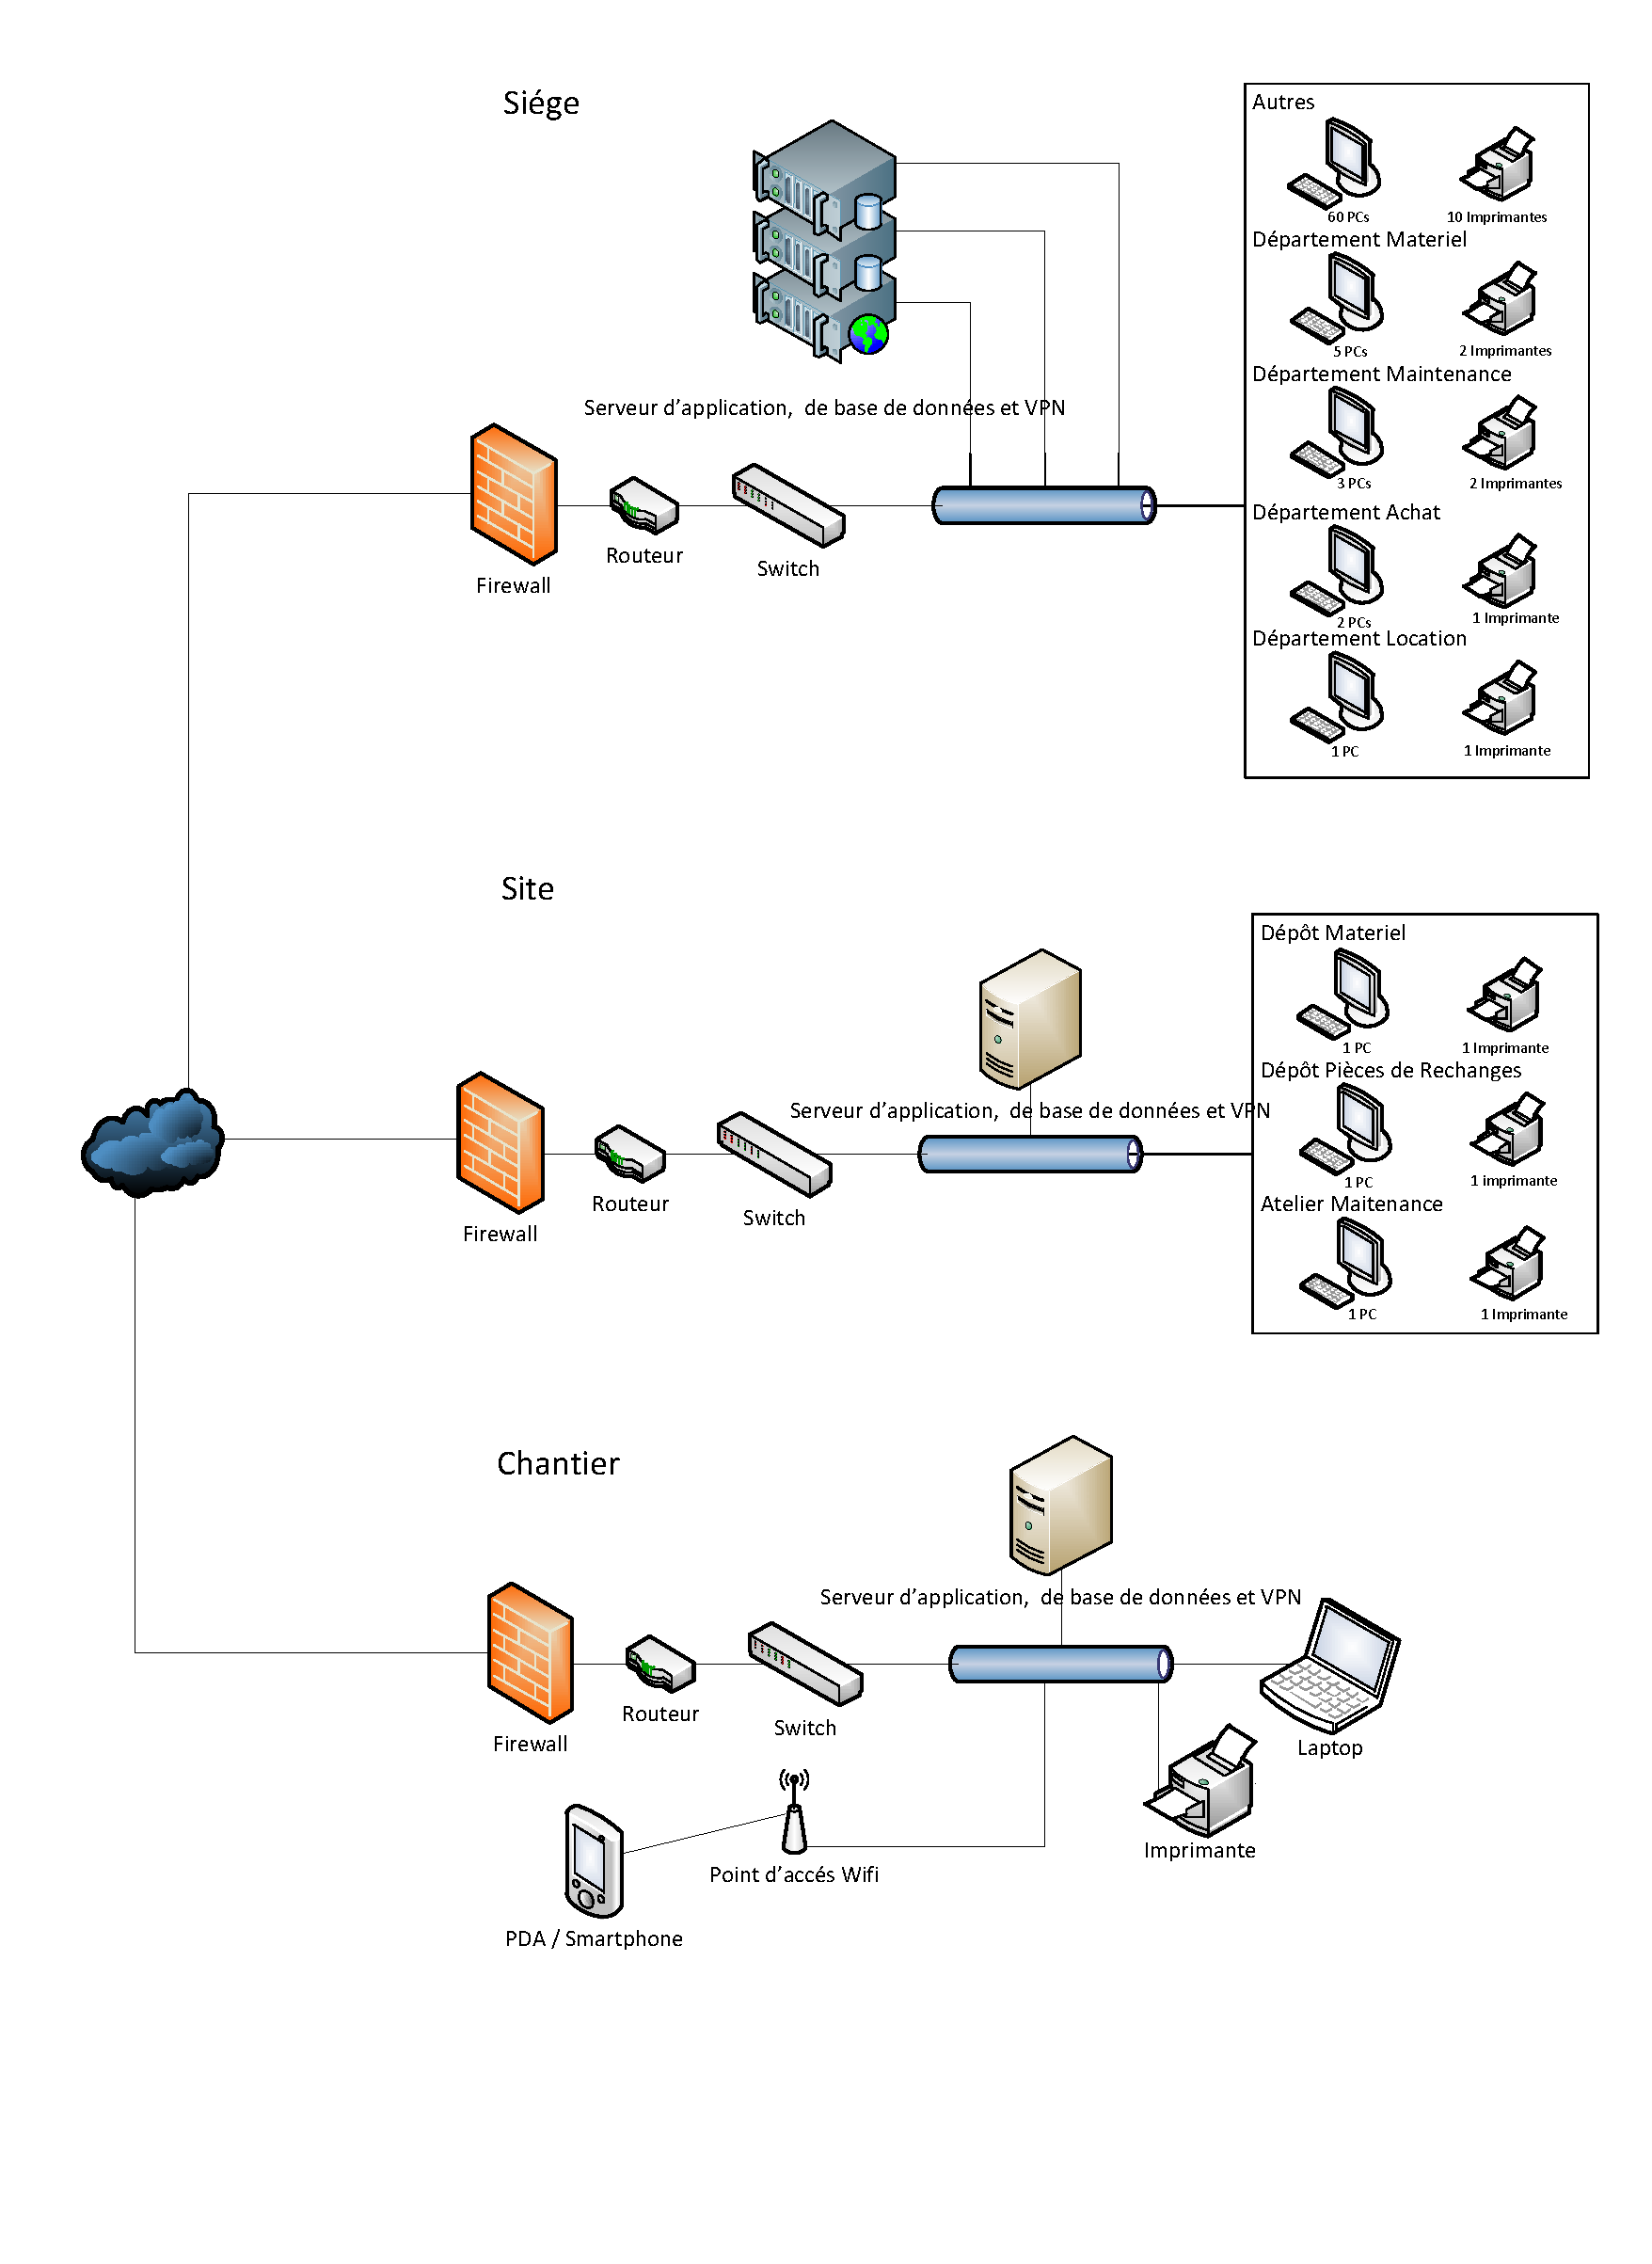
\includegraphics[width=0.9\textwidth]{img/schema-gstp.pdf}

\section{Mise en place de l'architecture téchnique}

    Notre solution de communication se basera principalement sur l'utilisation d'un VPN.

    Chaque site accueillera un serveur d'application, ce serveur aura à sa charge un serveur VPN fournissant à tout les clients un accès de type intranet identique sur tous les sites.
    Les terminaux mobiles auront également accès à ce VPN par le biais de connexion mobile, ou par wifi.

    Tous les clients se connecteront donc à ces serveurs à l'aide de clients VPN et profiterons ainsi d'un accès sécurisé à toutes les données nécessaires.

    Pour ce qui est du réseau, l'installation sera principalement impacté par la disposition des locaux.
    Dans tout les cas, on ne pourra se passer, par site, d'un firewall et d'un routeur, suivi d'un ou plusieurs switch permettant de distribuer le réseau dans chacune des infrastructures.

    Étant donné que la plupart des employé auront une grande mobilité, il peut être judicieux de les équiper uniquement de postes clients portables, ce qui sera fait d'ailleurs sur les chantiers.

    \subsection{Siége}

        \subsubsection{Serveur d'application / de données}
            Le siège hébergera la principale base de données. Cette dernière sera la plus performante possible, et résistera à des montées de charge. Le serveur sera de type rack et sera installé dans une salle dédié réfrigéré avec accès réglementé. Cette salle comportera également, le firewall, le routeur et le switch.

            Le besoin en stockage et en réactivité ne justifie pas l'utilisation de cluster, ni de base de données disjointe. Le choix le plus judicieux est donc un serveur unique performant et disposant d'une grande quantité de stockage. Pour une estimation du prix en vue d'un choix précis, on peut le borner très généreusement à 10 000€.
            Ce serveur sera le cœur de toutes l'installation, autrement dit il sera le plus critique, il est important qu'il soit de la meilleur qualité possible. Il permettras l'exécution du serveur VPN ainsi que de l'application.

        \subsubsection{Réseau : Firewall, Routeur et switch}
            Afin de connecter les postes clients au serveur, l'installation d'un réseau local est indispensable. Cette connexion se fera par l'intermédiaire d'un switch sur lequel le serveur et tous les postes clients se connecteront. Un routeur en amont permettra notamment la distribution d'adresse IP. Une estimation du prix du routeur et du switch nous a permis de chiffrer chacun d'eux à 1000€.
            Afin de connecter ce réseau local à l'extérieur, l'accès internet sera fourni par l'intermédiaire d'un firewall. Ce firewall sera de qualité professionnel, et sera aussi important que le serveur lui-même. Son prix est estimé à 1000€.
        
        \subsubsection{Postes clients}
            Il faut compter un poste client par utilisateur ayant besoin d'un ordinateur pour réaliser son travail. On compte 71 personnes sur le site central, donc 71 postes clients seront mis en place. Chaque service dispose d'une ou plusieurs imprimantes. 16 imprimantes seront mis en place (se référer au schéma pour la répartition exacte des postes et des imprimantes).

    \subsection{Sites secondaires}

        \subsubsection{Serveur d'application / de données}
            Tout comme le siège chacun des sites secondaire comportera un serveur hébergeant l'application, et un clone de la base de données du siège. Ces sites étant moins important en effectif, la charge sur le serveur sera donc moindre. Cependant, on peut s'attendre à une expansion de l'entreprise, il serait donc judicieux d'investir dans du matériel performant, sans être inutilement couteux. Le choix le plus judicieux sera probablement une tour simple dans une pièce unique réfrigéré avec accès réglementé. Comme sur le site principal, cette pièce hébergera le firewall, le routeur et le switch.

        \subsubsection{Réseau : Firewall, Routeur et switch}
            L'infrastructure sera sensiblement la même que sur le site principale, des détails pourront être apportés ultérieurement.

        \subsubsection{Postes clients}
            Il faut compter un poste client par service géré par chaque site secondaire, ainsi 3 ordinateurs et 3 imprimantes par site secondaire seront mis en place.

    \subsection{Chantier}
        L'architecture technique des chantier sera sensiblement la même que pour les sites secondaires.
        A la différence que chaque chantier pourras être équipé d'une borne d'accès wifi afin de facilité la connexion des smartphone à l'architecture applicative. Aussi un unique ordinateur sera mis en place sur chaque chantier.




